\documentclass[12pt, fullpage,letterpaper]{article}

\usepackage[margin=1in]{geometry}
\usepackage{url}
\usepackage{amsmath}
\usepackage{amssymb}
\usepackage{xspace}
\usepackage{graphicx}
\usepackage{hyperref}
\usepackage{cancel}
%\usepackage{graphicx}
%\usepackage{subfig}

\newcommand{\semester}{Spring 2022}
\newcommand{\assignmentId}{3}
\newcommand{\releaseDate}{15 Mar, 2022}
\newcommand{\dueDate}{11:59pm, 29 Mar, 2022}
\newcommand\independent{\protect\mathpalette{\protect\independenT}{\perp}}
\def\independenT#1#2{\mathrel{\rlap{$#1#2$}\mkern2mu{#1#2}}}

\newcommand{\bx}{{\bf x}}
\newcommand{\bw}{{\bf w}}

\title{CS 6190: Probabilistic Machine Learning \semester}
\author{Homework \assignmentId}
\date{Handed out: \releaseDate\\
  Due: \dueDate}

\begin{document}
\maketitle

% Math commands by Thomas Minka
\newcommand{\var}{{\rm var}}
\newcommand{\Tr}{^{\rm T}}
\newcommand{\vtrans}[2]{{#1}^{(#2)}}
\newcommand{\kron}{\otimes}
\newcommand{\schur}[2]{({#1} | {#2})}
\newcommand{\schurdet}[2]{\left| ({#1} | {#2}) \right|}
\newcommand{\had}{\circ}
\newcommand{\diag}{{\rm diag}}
\newcommand{\invdiag}{\diag^{-1}}
\newcommand{\rank}{{\rm rank}}
% careful: ``null'' is already a latex command
\newcommand{\nullsp}{{\rm null}}
\newcommand{\tr}{{\rm tr}}
\renewcommand{\vec}{{\rm vec}}
\newcommand{\vech}{{\rm vech}}
\renewcommand{\det}[1]{\left| #1 \right|}
\newcommand{\pdet}[1]{\left| #1 \right|_{+}}
\newcommand{\pinv}[1]{#1^{+}}
\newcommand{\erf}{{\rm erf}}
\newcommand{\hypergeom}[2]{{}_{#1}F_{#2}}

% boldface characters
\renewcommand{\a}{{\bf a}}
\renewcommand{\b}{{\bf b}}
\renewcommand{\c}{{\bf c}}
\renewcommand{\d}{{\rm d}}  % for derivatives
\newcommand{\e}{{\bf e}}
\newcommand{\f}{{\bf f}}
\newcommand{\g}{{\bf g}}
\newcommand{\h}{{\bf h}}
%\newcommand{\k}{{\bf k}}
% in Latex2e this must be renewcommand
\renewcommand{\k}{{\bf k}}
\newcommand{\m}{{\bf m}}
\newcommand{\mb}{{\bf m}}
\newcommand{\n}{{\bf n}}
\renewcommand{\o}{{\bf o}}
\newcommand{\p}{{\bf p}}
\newcommand{\q}{{\bf q}}
\renewcommand{\r}{{\bf r}}
\newcommand{\s}{{\bf s}}
\renewcommand{\t}{{\bf t}}
\renewcommand{\u}{{\bf u}}
\renewcommand{\v}{{\bf v}}
\newcommand{\w}{{\bf w}}
\newcommand{\x}{{\bf x}}
\newcommand{\y}{{\bf y}}
\newcommand{\z}{{\bf z}}
%s\newcommand{\l}{\boldsymbol{l}}
\newcommand{\A}{{\bf A}}
\newcommand{\B}{{\bf B}}
\newcommand{\C}{{\bf C}}
\newcommand{\D}{{\bf D}}
\newcommand{\E}{{\bf E}}
\newcommand{\F}{{\bf F}}
\newcommand{\G}{{\bf G}}
\renewcommand{\H}{{\bf H}}
\newcommand{\I}{{\bf I}}
\newcommand{\J}{{\bf J}}
\newcommand{\K}{{\bf K}}
\renewcommand{\L}{{\bf L}}
\newcommand{\M}{{\bf M}}
\newcommand{\N}{\mathcal{N}}  % for normal density
\newcommand{\Dcal}{\mathcal{D}}  % for normal density

%\newcommand{\N}{{\bf N}}
\renewcommand{\O}{{\bf O}}
\renewcommand{\P}{{\bf P}}
\newcommand{\Q}{{\bf Q}}
\newcommand{\R}{{\bf R}}
\renewcommand{\S}{{\bf S}}
\newcommand{\T}{{\bf T}}
\newcommand{\U}{{\bf U}}
\newcommand{\V}{{\bf V}}
\newcommand{\W}{{\bf W}}
\newcommand{\X}{{\bf X}}
\newcommand{\Y}{{\bf Y}}
\newcommand{\Z}{{\bf Z}}

% this is for latex 2.09
% unfortunately, the result is slanted - use Latex2e instead
%\newcommand{\bfLambda}{\mbox{\boldmath$\Lambda$}}
% this is for Latex2e
\newcommand{\bfLambda}{\boldsymbol{\Lambda}}

% Yuan Qi's boldsymbol
\newcommand{\bsigma}{\boldsymbol{\sigma}}
\newcommand{\balpha}{\boldsymbol{\alpha}}
\newcommand{\bpsi}{\boldsymbol{\psi}}
\newcommand{\bphi}{\boldsymbol{\phi}}
\newcommand{\boldeta}{\boldsymbol{\eta}}
\newcommand{\Beta}{\boldsymbol{\eta}}
\newcommand{\btau}{\boldsymbol{\tau}}
\newcommand{\bvarphi}{\boldsymbol{\varphi}}
\newcommand{\bzeta}{\boldsymbol{\zeta}}

\newcommand{\blambda}{\boldsymbol{\lambda}}
\newcommand{\bLambda}{\mathbf{\Lambda}}
\newcommand{\bOmega}{\mathbf{\Omega}}
\newcommand{\bomega}{\mathbf{\omega}}
\newcommand{\bPi}{\mathbf{\Pi}}

\newcommand{\btheta}{\boldsymbol{\theta}}
\newcommand{\bpi}{\boldsymbol{\pi}}
\newcommand{\bxi}{\boldsymbol{\xi}}
\newcommand{\bSigma}{\boldsymbol{\Sigma}}

\newcommand{\bgamma}{\boldsymbol{\gamma}}
\newcommand{\bGamma}{\mathbf{\Gamma}}

\newcommand{\bmu}{\boldsymbol{\mu}}
\newcommand{\1}{{\bf 1}}
\newcommand{\0}{{\bf 0}}

% \newcommand{\comment}[1]{}

\newcommand{\bs}{\backslash}
\newcommand{\ben}{\begin{enumerate}}
\newcommand{\een}{\end{enumerate}}

 \newcommand{\notS}{{\backslash S}}
 \newcommand{\nots}{{\backslash s}}
 \newcommand{\noti}{{\backslash i}}
 \newcommand{\notj}{{\backslash j}}
 \newcommand{\nott}{\backslash t}
 \newcommand{\notone}{{\backslash 1}}
 \newcommand{\nottp}{\backslash t+1}
% \newcommand{\notz}{\backslash z}

\newcommand{\notk}{{^{\backslash k}}}
%\newcommand{\noti}{{^{\backslash i}}}
\newcommand{\notij}{{^{\backslash i,j}}}
\newcommand{\notg}{{^{\backslash g}}}
\newcommand{\wnoti}{{_{\w}^{\backslash i}}}
\newcommand{\wnotg}{{_{\w}^{\backslash g}}}
\newcommand{\vnotij}{{_{\v}^{\backslash i,j}}}
\newcommand{\vnotg}{{_{\v}^{\backslash g}}}
\newcommand{\half}{\frac{1}{2}}
\newcommand{\msgb}{m_{t \leftarrow t+1}}
\newcommand{\msgf}{m_{t \rightarrow t+1}}
\newcommand{\msgfp}{m_{t-1 \rightarrow t}}

\newcommand{\proj}[1]{{\rm proj}\negmedspace\left[#1\right]}
\newcommand{\argmin}{\operatornamewithlimits{argmin}}
\newcommand{\argmax}{\operatornamewithlimits{argmax}}

\newcommand{\dif}{\mathrm{d}}
\newcommand{\abs}[1]{\lvert#1\rvert}
\newcommand{\norm}[1]{\lVert#1\rVert}

%miscellaneous symbols
\newcommand{\ie}{{{i.e.,}}\xspace}
\newcommand{\eg}{{{\em e.g.,}}\xspace}
\newcommand{\EE}{\mathbb{E}}
\newcommand{\VV}{\mathbb{V}}
\newcommand{\sbr}[1]{\left[#1\right]}
\newcommand{\rbr}[1]{\left(#1\right)}
\newcommand{\cmt}[1]{}



\footnotesize
	\begin{itemize}
		\item You are welcome to talk to other members of the class about
		the homework. I am more concerned that you understand the
		underlying concepts. However, you should write down your own
		solution. Please keep the class collaboration policy in mind.
		
		\item Feel free discuss the homework with the instructor or the TAs.
		
		\item Your written solutions should be brief and clear. You need to
		show your work, not just the final answer, but you do \emph{not}
		need to write it in gory detail. Your assignment should be {\bf no
			more than 10 pages}. Every extra page will cost a point.
		
		\item Handwritten solutions will not be accepted.
		
		\item The homework is due by \textbf{midnight of the due date}. Please submit
		the homework on Canvas.
	\end{itemize}



\section*{Analytical problems [100 points + 40 bonus]}	
\label{sec:q1}
%1. show Jeffery's prior for Gaussian
%2. show Jeffern's prior for Poisson 
\begin{enumerate}
\item~[13 points] The joint distribution over three binary variables are given in Table \ref{tb:abc}. Show by direct evaluation that this distribution has the property that $a$ and $b$ are marginally dependent, so that $p(a, b) \neq p(a)p(b)$, but that they become independent conditioned on $c$, \ie  $p(a,b|c) = p(a|c)p(b|c)$. 
\begin{table}
	\centering
	\begin{tabular}{c|c|c|c}
		\hline
		a & b & c  & p(a,b,c)\\
		\hline
		0 & 0 & 0 & 0.192\\
		0 & 0 & 1 & 0.144\\
		0 & 1 & 0 & 0.048\\
		0 & 1 & 1 & 0.216\\
	    1 & 0 & 0 & 0.192\\
	    1 & 0 & 1  & 0.064\\
	    1 & 1 & 0 & 0.048\\
	    1 & 1 & 1 & 0.096\\
	    \hline
	\end{tabular}
\caption{Joint distribution of $a,b,c$.} \label{tb:abc}
\end{table}

\item~[12 points] Using the d-separation algorithm/criterion (Bayes ball algorithm) to show that the conditional distribution for a node $x$ in a directed graph, conditioned on all of the nodes in its Markov blanket, is independent of the remaining variables in the graph.



\begin{figure}[h]
\centering
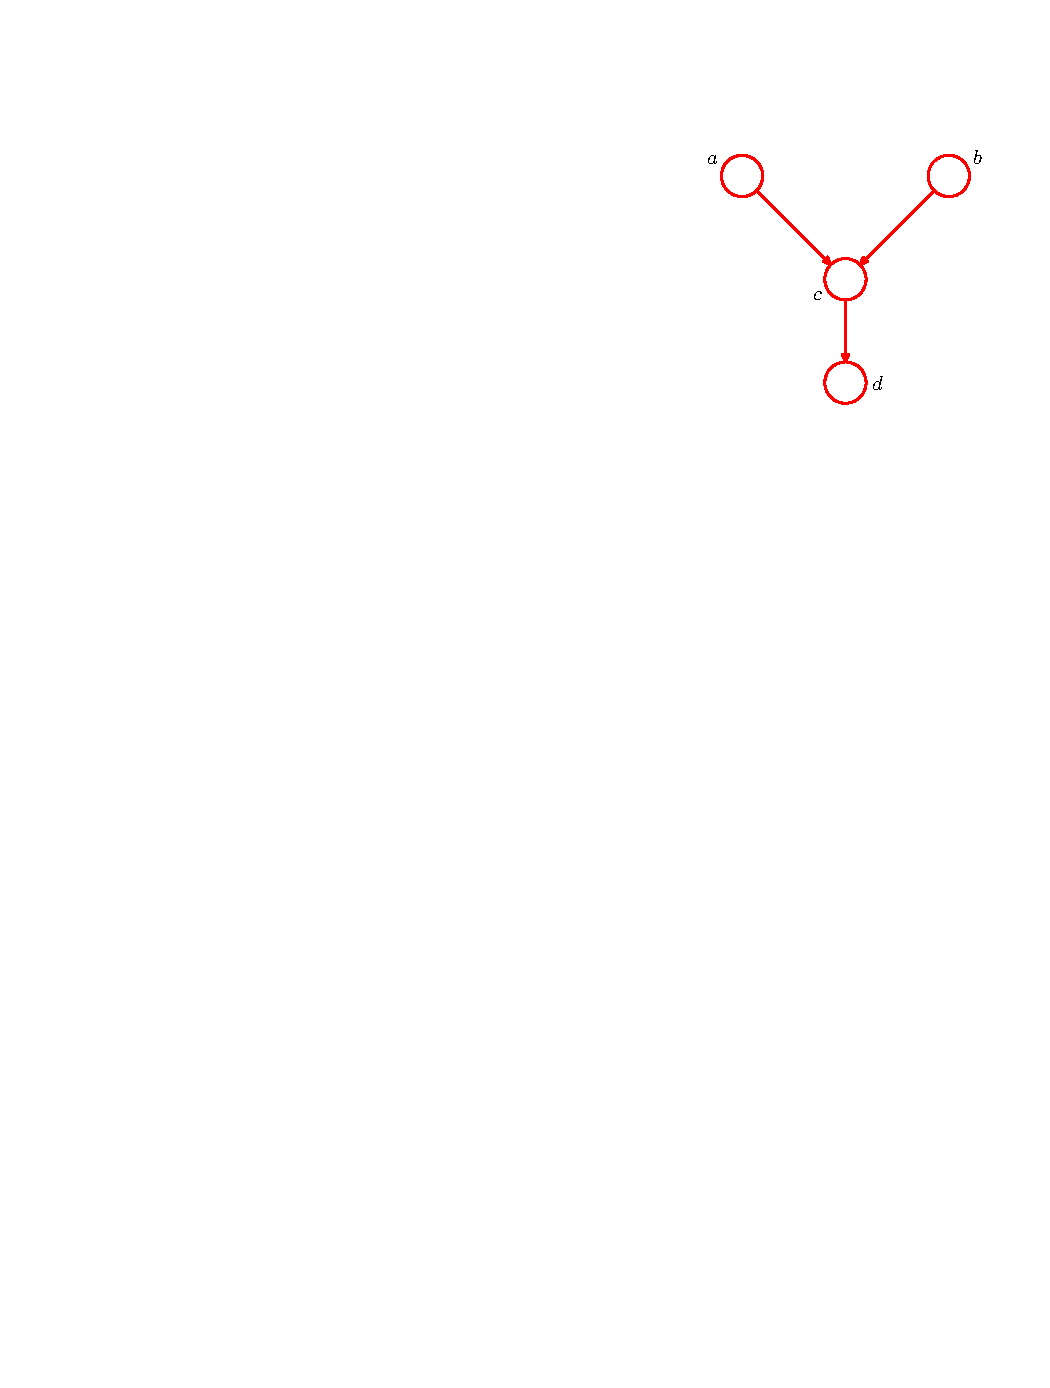
\includegraphics[width=0.3\linewidth]{./fig1.pdf} 
\caption{Graphical model.} \label{fig:graph}
\end{figure}

\item~[15 points] See the graphical model in Figure \ref{fig:graph}. Recall what we have discussed in the class. Show that $a \independent b | \emptyset $. Suppose we have observed the variable $d$. Show that in general $a \cancel{ \independent} b | d$.

\item~[10  points] Convert the directed graphical model in Figure \ref{fig:graph} into an undirected graphical model. Draw the structure and write down the definition of the potential functions. 

\item~[15 points] Write down every step of the sum-product algorithm for the graphical model shown in Figure \ref{fig:graph2}. Note that you need to first choose a root node, and write down how to compute each message. Once all your messages are ready, please explain how to compute the marginal distribution $p(x_4, x_5)$.

\begin{figure}[h]
	\centering
	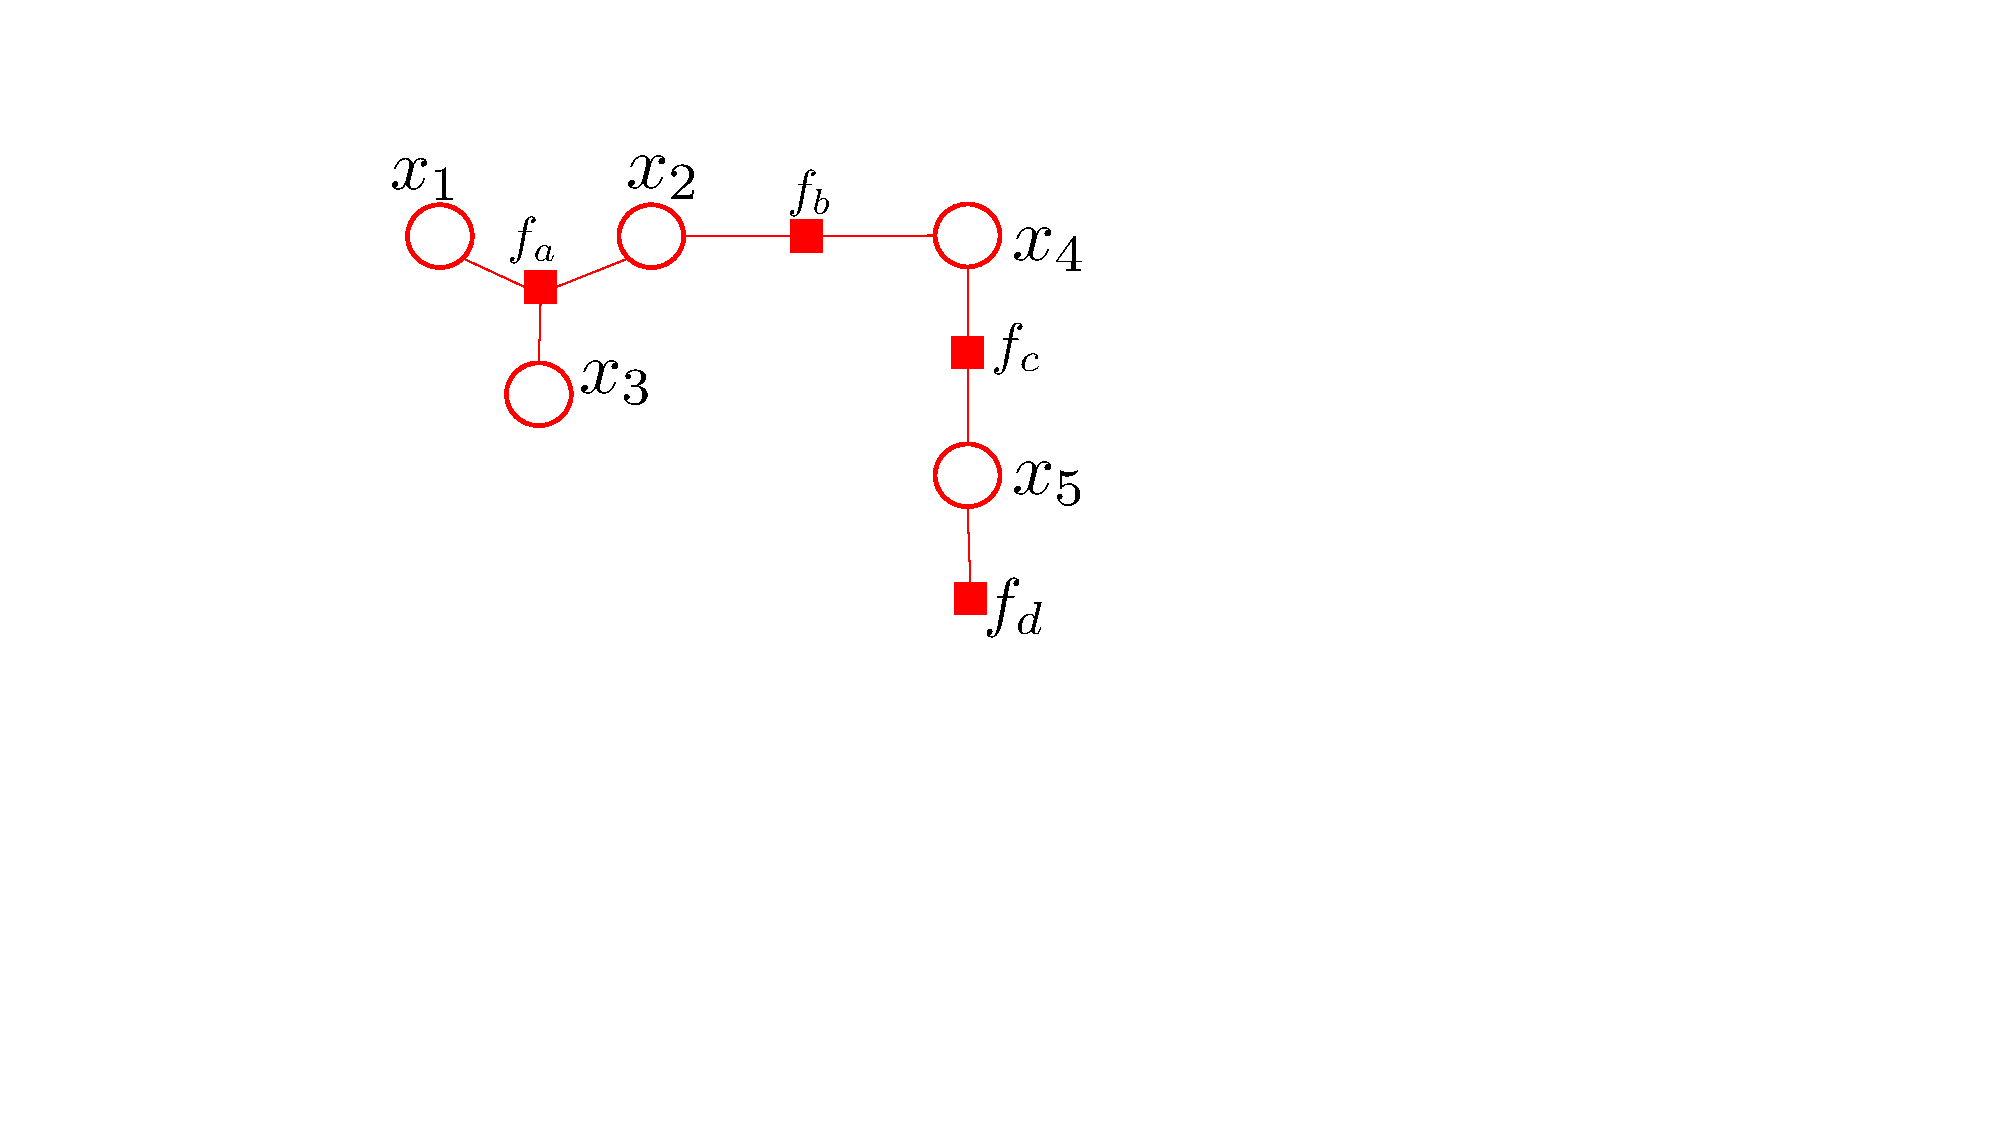
\includegraphics[width=0.4\linewidth]{./fig2.pdf} 
	\caption{Factor graph.} \label{fig:graph2}
\end{figure}


\item~[10 points] Now if $x_2$ in Figure \ref{fig:graph2} is observed, explain how to conduct the sum-product algorithm, and compute the posterior distribution $p(x_4, x_5|x_2)$.

\item~[10 points] Suppose all the random variables in Figure \ref{fig:graph2} are discrete, and no one has been observed. Now we want to find the configuration of the $x_1, \ldots, x_5$ to maximize the joint probability. Write done every step of the max-sum algorithm to calculate the maximum joint probability and to find the corresponding configurations of each random variable. 


\item~[\textbf{Bonus}][20 points] Show the message passing protocol we discussed in the class is always valid on the tree-structured graphical models--- whenever we compute a message (from a factor to a variable or a variable to a factor), the dependent messages are always available. Hint: use induction. 

\begin{figure}[h]
	\centering
	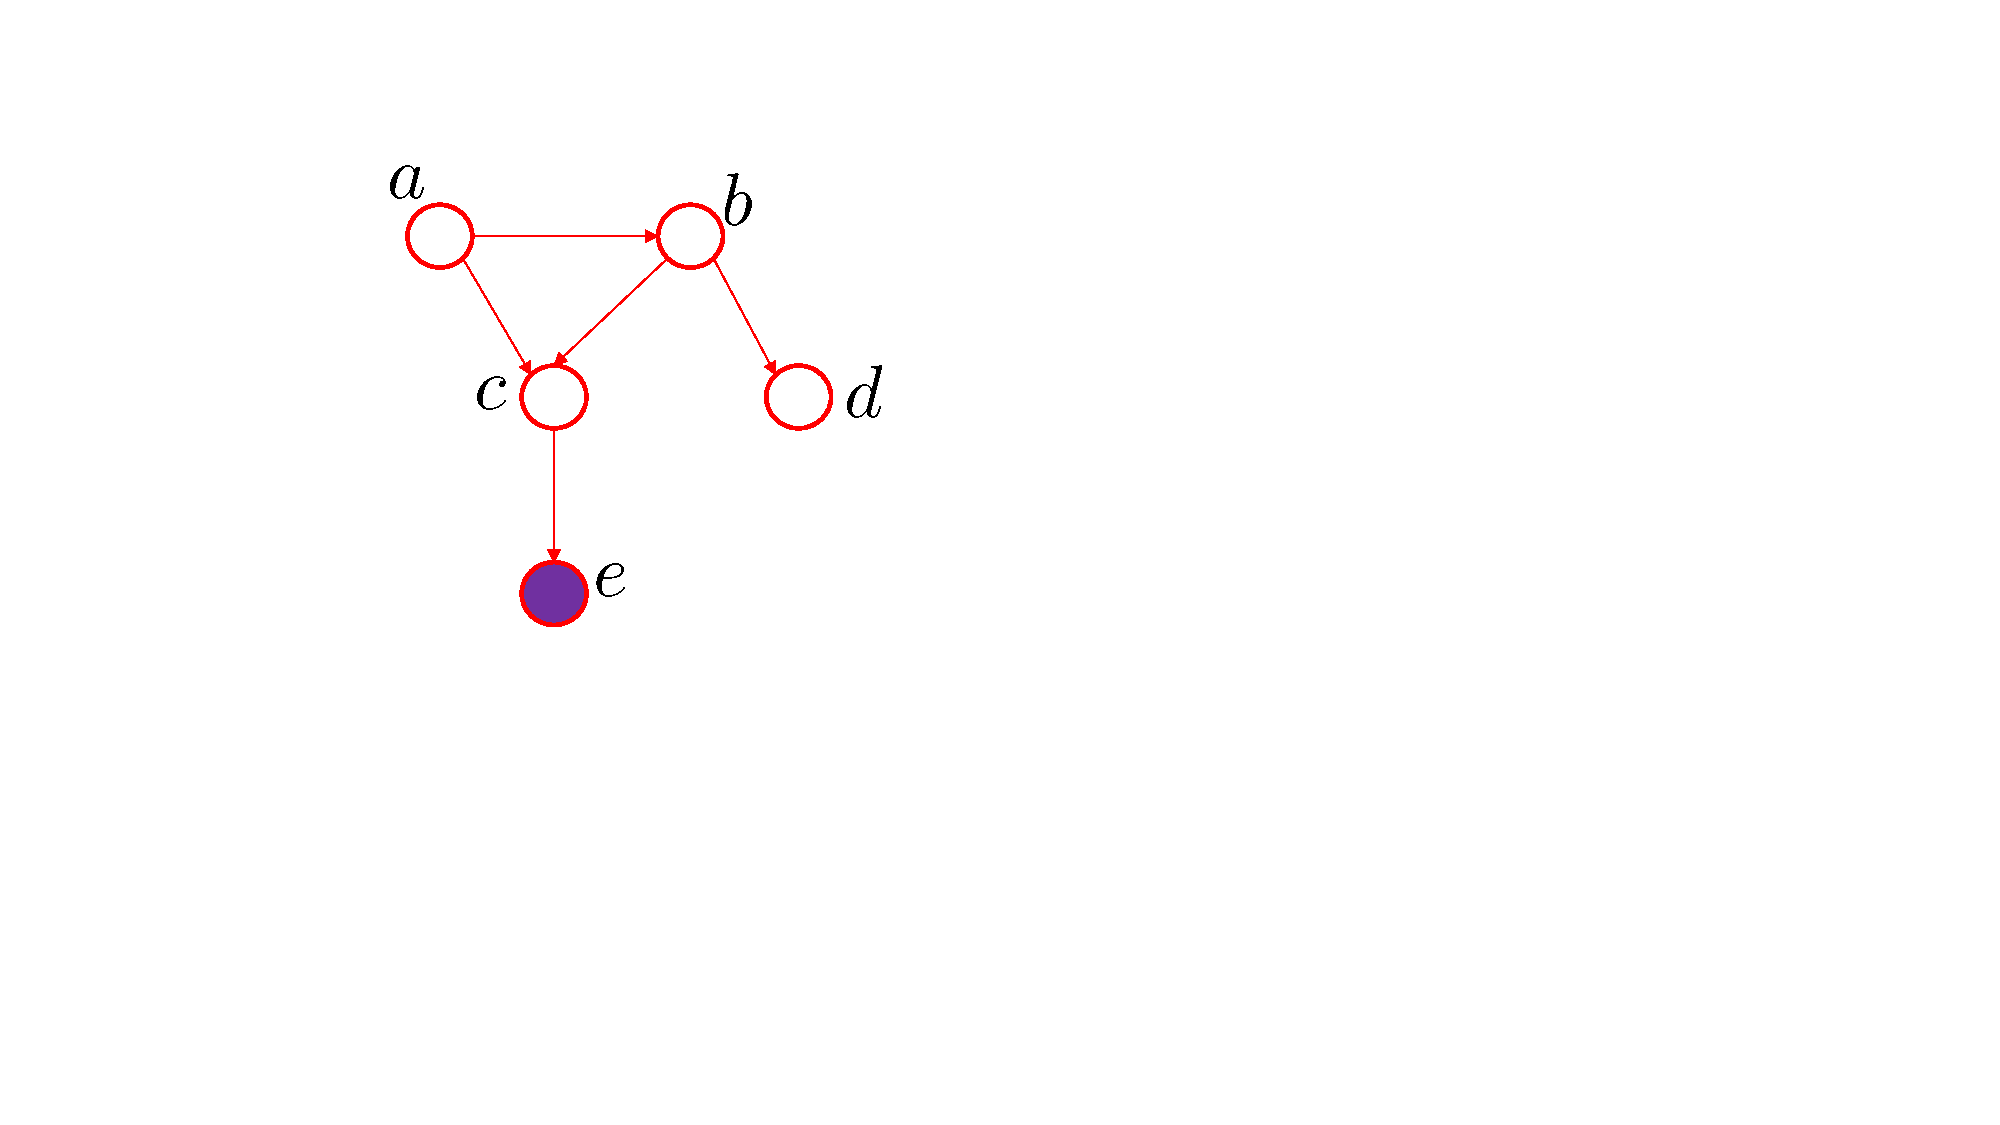
\includegraphics[width=0.4\linewidth]{./fig3_1.pdf} 
	\caption{Model 1.} \label{fig:graph3}
\end{figure}
\begin{figure}[h]
	\centering
	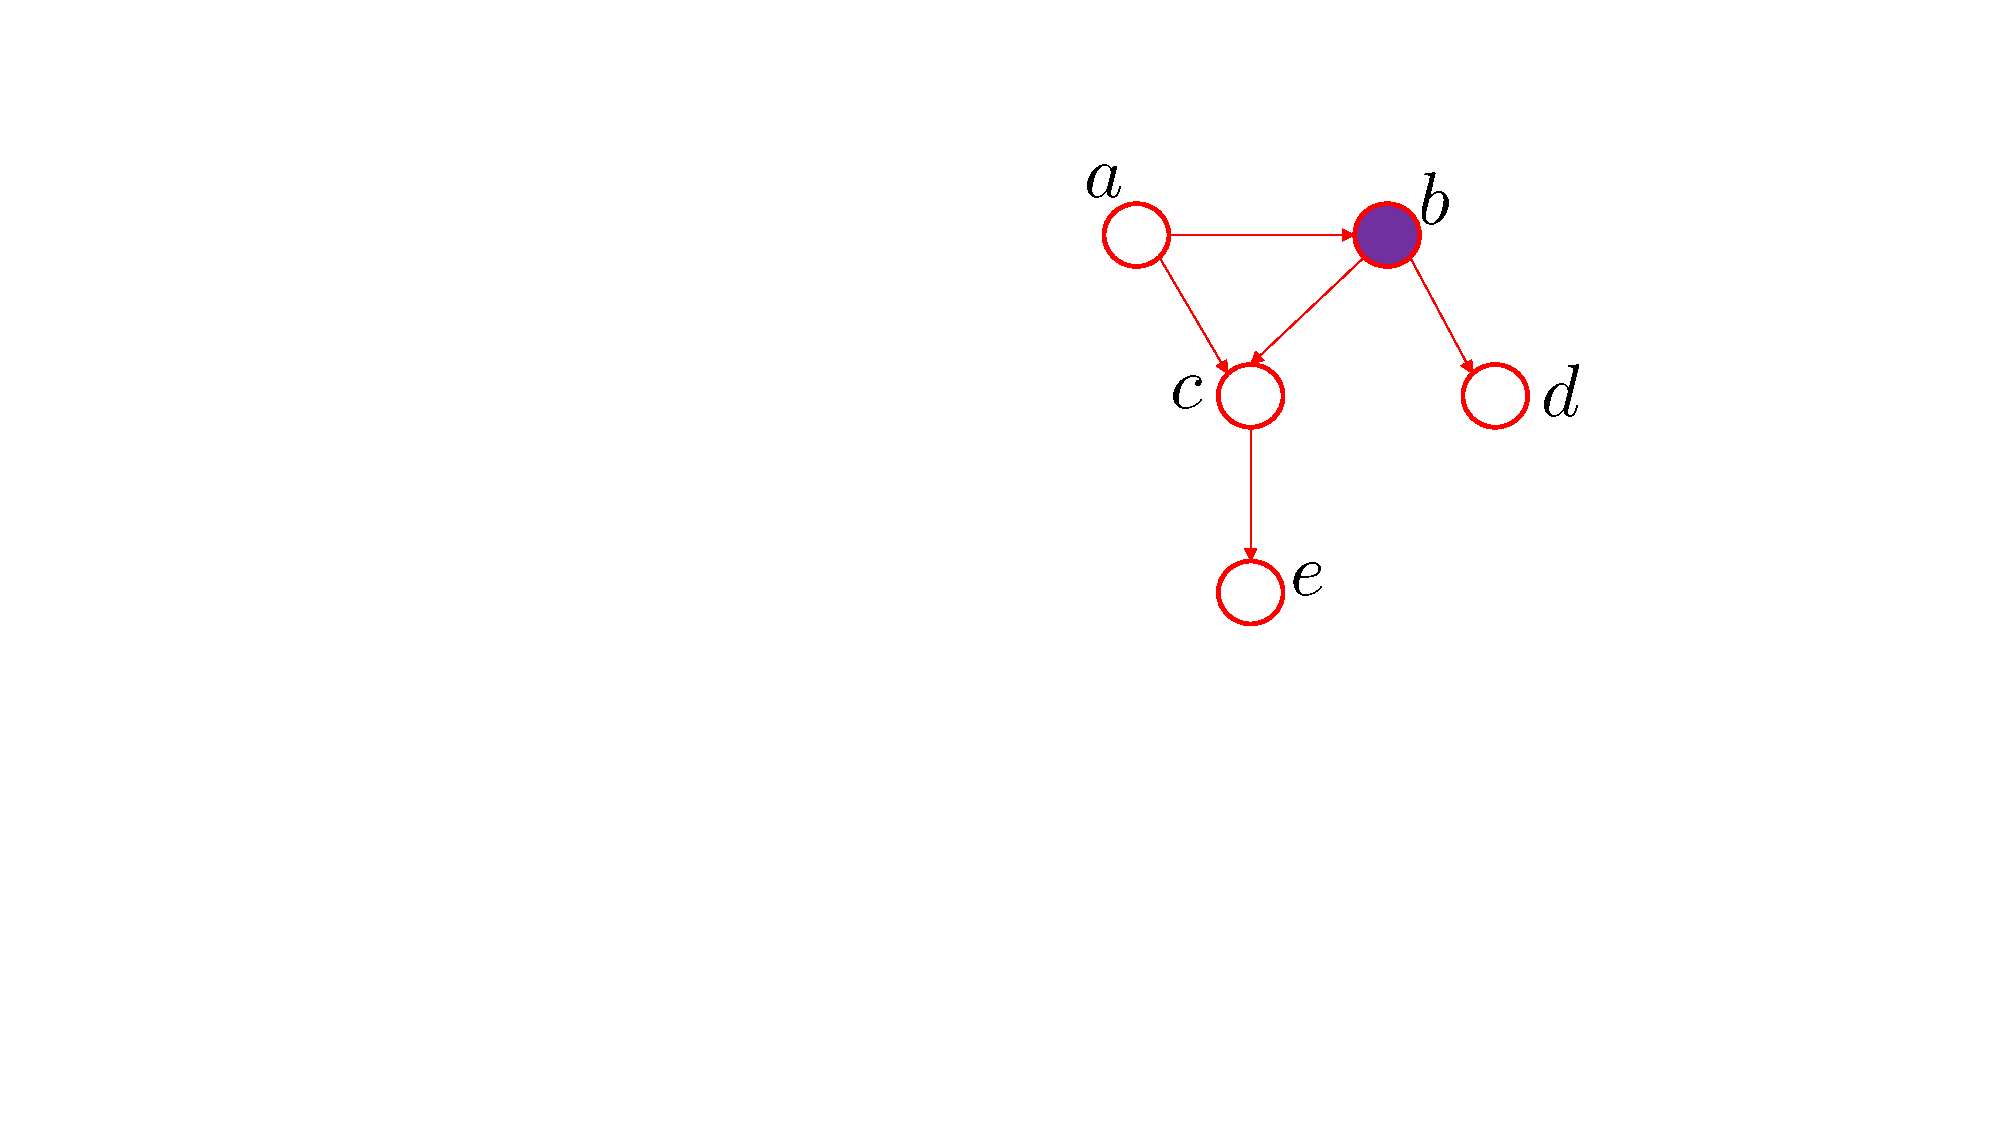
\includegraphics[width=0.4\linewidth]{./fig3_2.pdf} 
	\caption{Model 2.} \label{fig:graph4}
\end{figure}


\item~[15 points] Use d-separation algorithm (Bayes ball) to determine if $a \independent d | e$ in the graphical  model shown in Figure \ref{fig:graph3}, and if $a \independent d | b$ in the graphical model  shown in Figure  \ref{fig:graph4}. 

\begin{figure}[h]
	\centering
	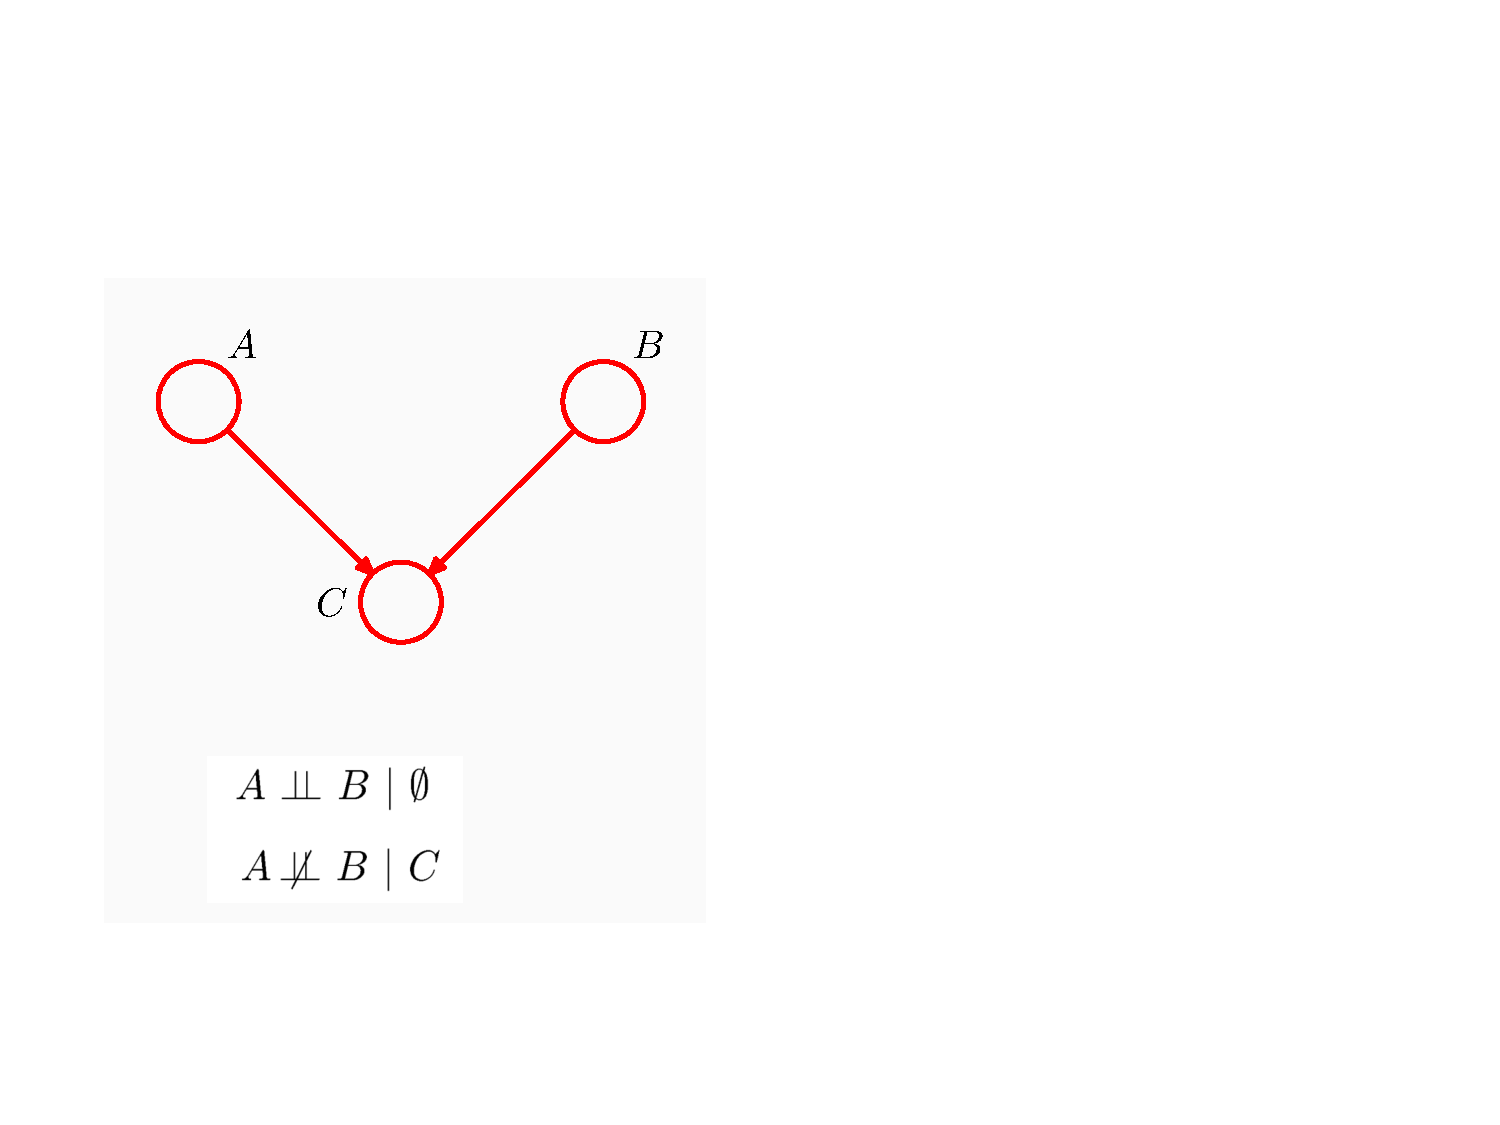
\includegraphics[width=0.4\linewidth]{./fig4.pdf} 
	\caption{Directed.} \label{fig:graph5}
\end{figure}
\begin{figure}[h]
	\centering
	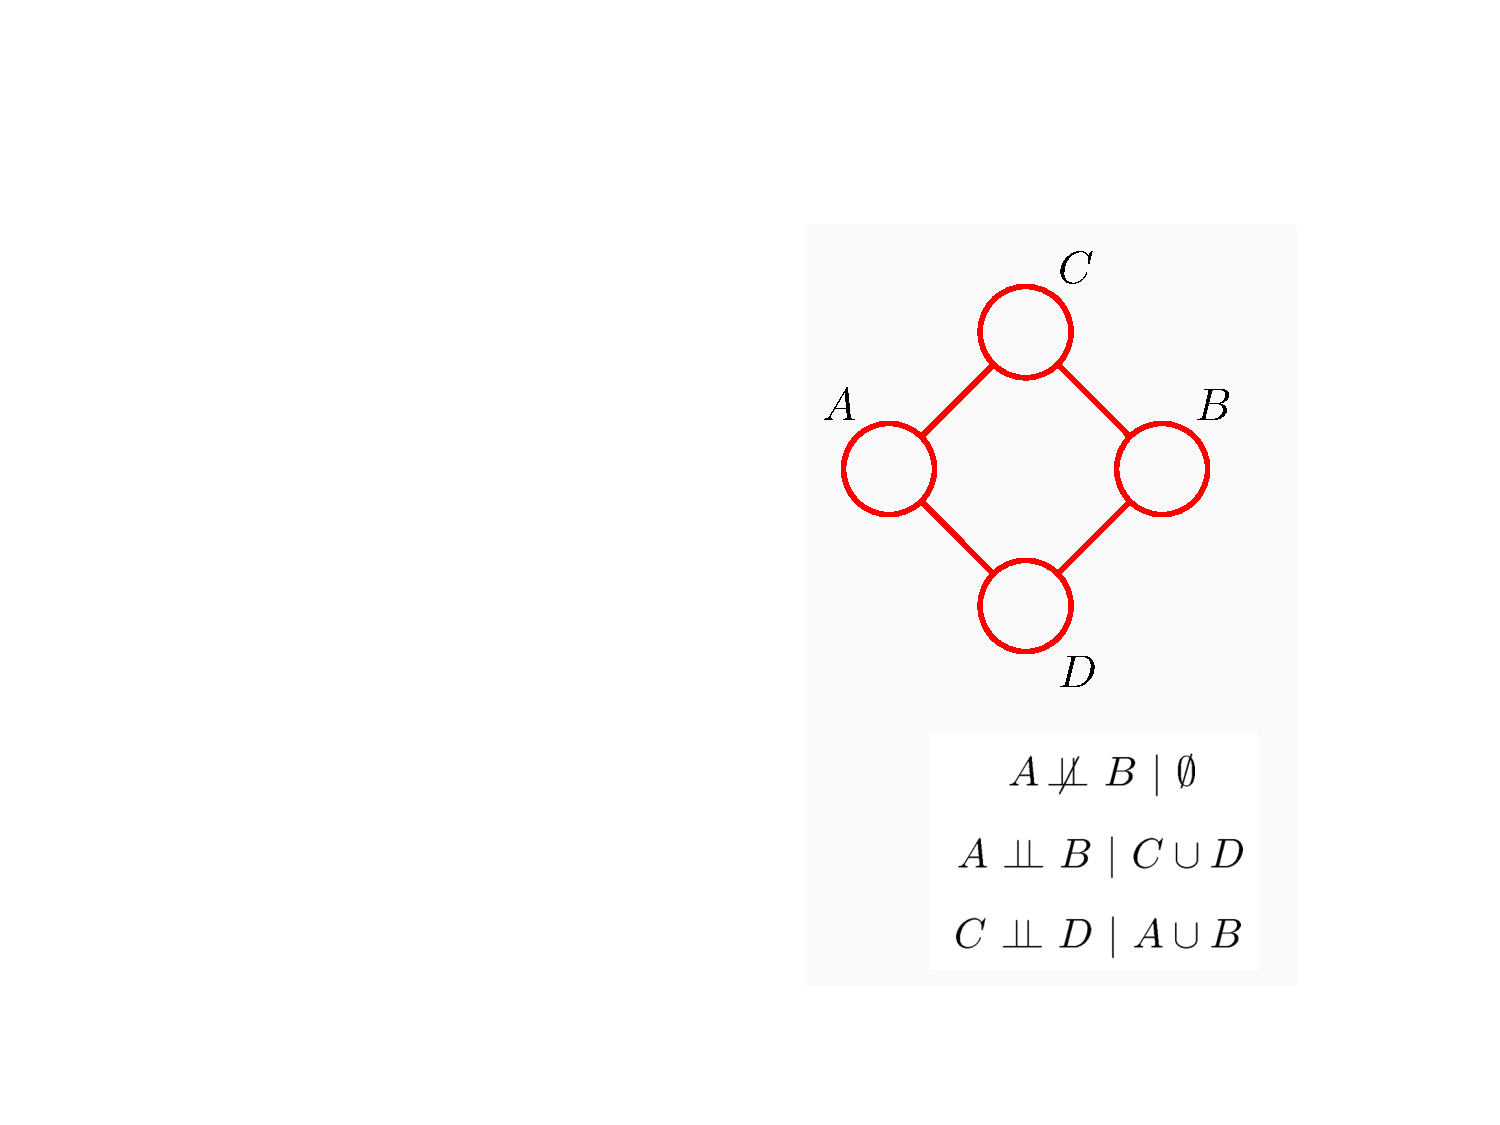
\includegraphics[width=0.4\linewidth]{./fig5.pdf} 
	\caption{Undirected.} \label{fig:graph6}
\end{figure}

\item~[\textbf{Bonus}][20 points] We have listed two examples in the class to  show that in terms of the expressiveness (i.e., conditional independence) of the directed and undirected graphical models , there is not a guarantee that who is better than who. 
\begin{enumerate}
	\item~[10 points] Now show that for the directed graphical model in Figure \ref{fig:graph5}, we cannot find an equivalent undirected graphical model to express the same set of conditional independence.
	\item~[10 points] Show that for the undirected graphical model in Figure \ref{fig:graph6}, we cannot find an equivalent directed graphical model to express the same set of conditional independence. 
\end{enumerate}


\end{enumerate}

\end{document}
